\chapter{Lösung häufiger Probleme}
Bei dem Druck von 3D-Modellen können viele verschiedene Probleme auftreten. Im Folgenden wurden drei der häufigsten Probleme herausgegriffen und deren Ursache sowie Lösung näher erläutert.

\begin{figure}[h]
  \centering
  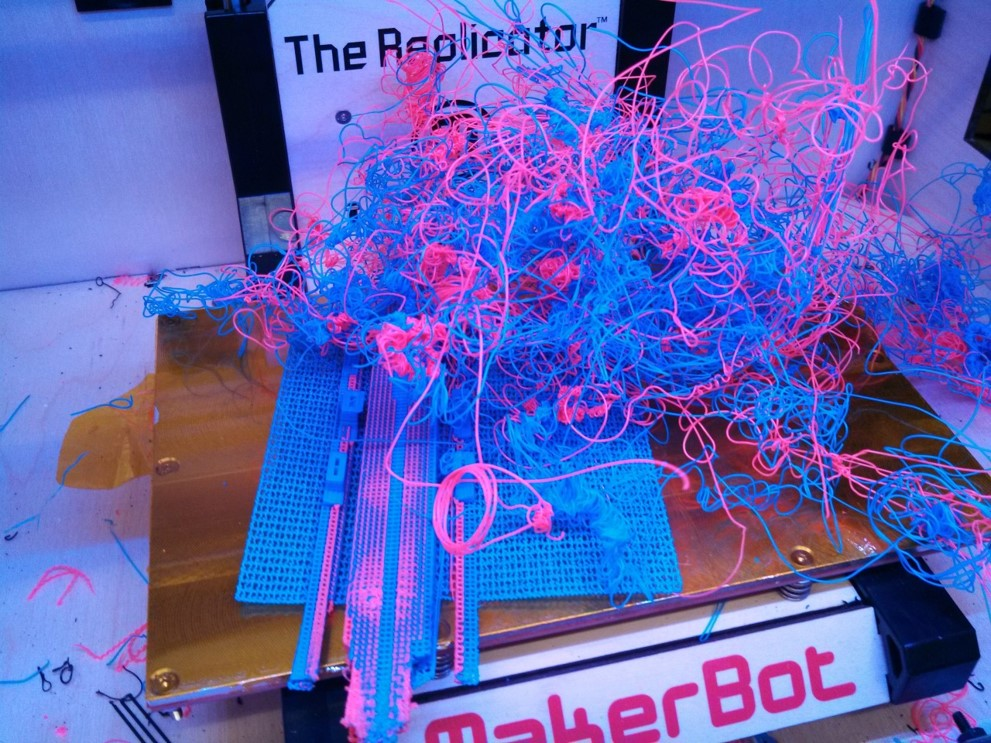
\includegraphics[width=14cm]{kapitel4/fail}
  \caption{Beispiel für einen fehlgeschlagenen 3D-Druck}
  \source{\url{http://epic3dprintingfail.tumblr.com/image/60950463852}}
  \label{Kap4:PrintFail}
\end{figure}

\section{Drooping}
Bei sog. \textit{Drooping} handelt es sich um herunterhängende Materialfäden, die bei dem Druck von Brücken oder Überhängen entstehen. Diesem kann durch die Verwendung von Supports entgegengewirkt werden. Sollte dies nicht möglich sein ist auch ein Verringern der Drucktemperatur oder die Verwendung eines anderen Materials denkbar.

\begin{figure}[h]
  \centering
  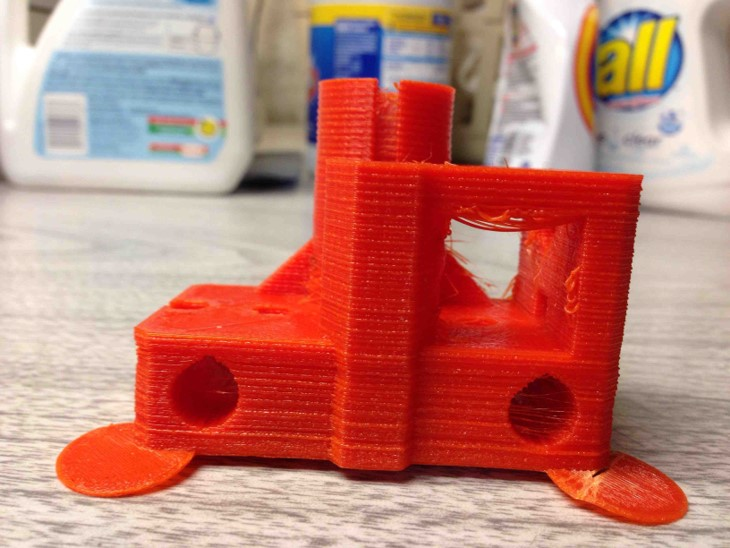
\includegraphics[width=14cm]{kapitel4/drooping}
  \caption{Beispiel für Drooping}
  \source{\url{https://imgur.com/wcRyGyS}}
  \label{Kap4:Drooping}
\end{figure}

\clearpage

\section{Warping}
Als \textit{Warping} wird die unregelmäßige Verformung des gedruckten Objektes während des Abkühlens bezeichnet, zu diesem Problem kommt es bei \ac{ABS} besonders häufig, weshalb es in einer geschlossenen Kammer und mit beheiztem Druckbett verarbeitet werden muss. Weitere Möglichkeiten sind die Verwendung eines Rafts oder der Wechsel zu einem anderen Material.

\begin{figure}[h]
  \centering
  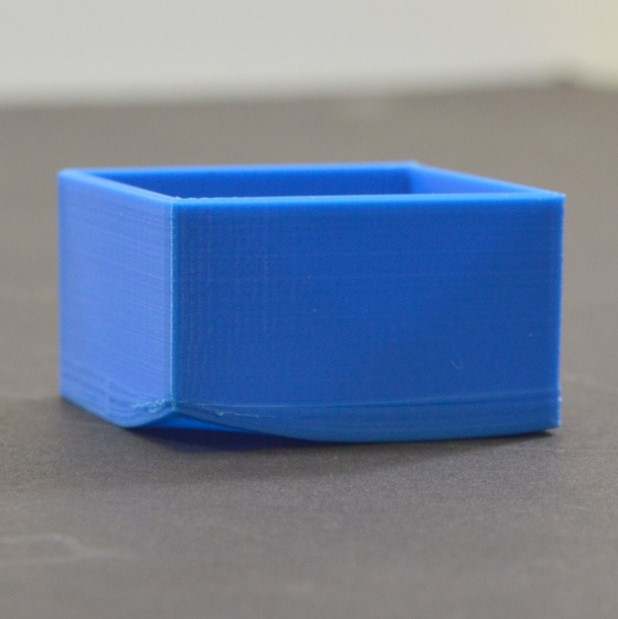
\includegraphics[width=14cm]{kapitel4/warping}
  \caption{Beispiel für Warping}
  \source{\url{https://www.simplify3d.com/support/print-quality-troubleshooting/}}
  \label{Kap4:Warping}
\end{figure}

\clearpage

\section{Stringing}
Zieht der Druckkopf während der Bewegung zwischen den Druckpositionen spinnennetzartige, dünne Fäden so handelt es sich um \textit{Stringing}. Dies lässt sich sehr einfach durch das Setzen einer größeren \textit{Retraction} vermeiden. Hierbei wird das Material während Bewegungen zwischen Druckpositionen aus dem Druckkopf gezogen um ein versehentliches Austreten zu verhindern. Auch eine Verringerung der Drucktemperatur kann dabei Abhilfe schaffen.

\begin{figure}[h]
  \centering
  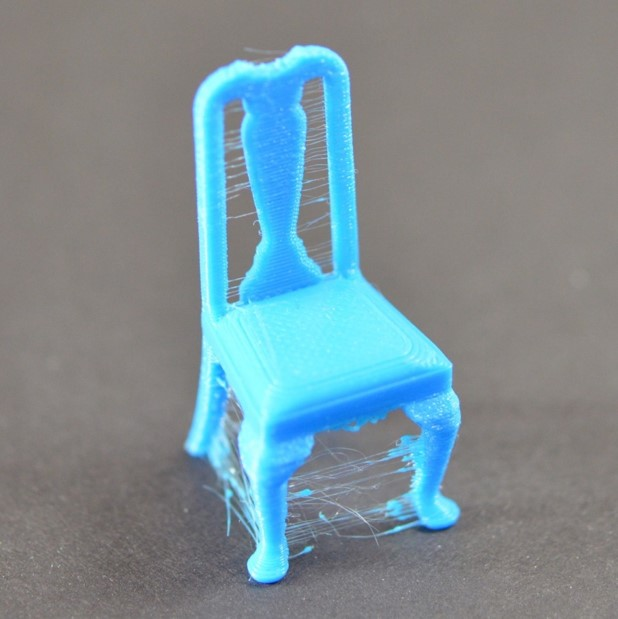
\includegraphics[width=14cm]{kapitel4/stringing}
  \caption{Beispiel für Stringing}
  \source{\url{https://www.simplify3d.com/support/print-quality-troubleshooting/}}
  \label{Kap4:Stringing}
\end{figure}